\documentclass{article}

\usepackage{graphicx}
\usepackage{amsmath}
\usepackage{amsbsy}

\renewcommand{\baselinestretch}{1.5}
\setlength{\topmargin}{-0.125 in}
\setlength{\oddsidemargin}{-0.125 in}
\setlength{\evensidemargin}{-0.125 in}
\setlength{\headheight}{0 in}
\setlength{\headsep}{0 in}
\setlength{\topskip}{0 in}
\setlength{\textheight}{9.3 in}
\setlength{\textwidth}{6.8 in}
\setlength{\parindent}{1cm}

\title{R or Python for Data Analysis?}
\author{Katherine Encarnacion, kencarnacion.student@manhattan.edu}
\date{\today}
\begin{document}
\maketitle
\indent Previously I had used R for data analysis purposes while completing midterm 2. I was hoping to replicate the midterm that focused mainly on data analysis using Python. Overall using Python was quite interesting even though it was frustrating at times, which is to be expected when learning to use any programming language. Python is an object-orientated programming language that as I have come to learn it contains many libraries that allow the syntax of your program to be very neat. Pandas is one of the libraries that Python contains, it is used for data structures and functions. Within Pandas it uses features of another library of Python called NumPy, which stands for Numerical Python, for data manipulation. Pandas also includes relational databases such as SQL [1].  As stated by McKinney,  ``Python’s improved library support (primarily pandas) has made it a strong alternative for data manipulation tasks. Combined with Python’s strength in general purpose programming, it is an excellent choice as a single language for building data-centric applications" [1]. With time and practice I think that Python has many different aspects to it that would be very useful to learn. The fact that it is a program that is mainly used by web programmers it has a sort of elegance when it comes to the syntax. 


\indent Prior to me trying to learn Python I briefly had some experience in R with data analysis. R is a statistical computing and graphing program.  ``R provides a wide variety of statistical (linear and nonlinear modelling, classical statistical tests, time-series analysis, classification, clustering, …) and graphical techniques, and is highly extensible" [2].  Many people believe that R is only for statistical purpose but it is not, just like Python it contains many libraries that can be integrated within your code to facilitate what you are trying to do. ``R is an integrated suite of software facilities for data manipulation, calculation and graphical display" [2]. It contains an environment which facilitates the way you access data frames. By simply clicking on a data frame in the environment it access a new window with the data frame being displayed. 


\indent In reproducing midterm 2 in Python I had to import four libraries: pandas, NumPy, csv, and matplotlib (figure 1). As explained previously NumPy, Numerical Python, is used for scientific computation. It allows for a more efficient way to manipulate data and sort arrays [1]. Which because of this I used NumPy within my code which allowed for a much easier and simpler way to extract values from an array using this package. Pandas is an add on to NumPy and allows you to create data frames. Within my code I used pandas to create data frames and subsets of various data frames. Also, when importing a csv into Python it is imported in as a data frame. I used csv within my code to create an excel csv file. Matplotlib is a library used to plot 2D figures. I used this library to produce the plot in problem 1 from midterm 2.

\begin{figure}[h]
\begin{center}
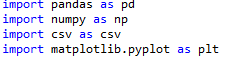
\includegraphics[width=0.4\textwidth]{import.png}
\end{center}
\caption{Import of Python libraries and package}
\end{figure}

\newpage

\indent For problem 1 we had to look at a data frame named ``heart.rate" (figure 2) and create a data frame with the average heart rate for each patient. It took a while to figure out how to make a data frame, especially since the syntax in “Python for Data Analysis” was incorrect (figure 3) because you have to include `$pd$' before `$DataFrame$'. After, finally understanding how to separate the heart rate by subject it was really easy to calculate the mean. In R I used the `$tapply$' function to calculate the mean of the various subjects and in Python you just have to put `$.mean()$' after the variable I used to group the subjects in the data frame. The way R and Python display data frames are very different. R creates a new window where you can see the data frame, while Python displays it in the console. But Python is very good at keeping the column names even after you group them to calculate the mean.


\begin{figure}[h]
\begin{center}
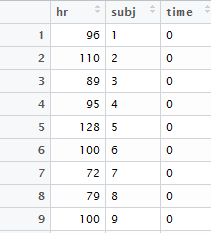
\includegraphics[width=0.2\textwidth]{heartratedata.png}
\end{center}
\caption{Part of the heart.rate data frame}
\end{figure}

\begin{figure}[h]
\begin{center}
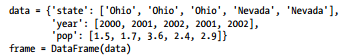
\includegraphics[width=0.6\textwidth]{dataframe.png}
\end{center}
\caption{Incorrect data frame syntax}
\end{figure}

\begin{figure}[h]
\begin{center}
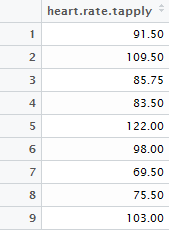
\includegraphics[width=0.2\textwidth]{displayP1R.png}
\end{center}
\caption{Display of R data frame for problem 1}
\end{figure}


\begin{figure}[h]
\begin{center}
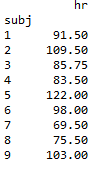
\includegraphics[width=0.2\textwidth]{displayP1Python.png}
\end{center}
\caption{Display of Python data frame for problem 1}
\end{figure}

\newpage
\indent For problem 2 I had to create factors for the data of the blood.glucose variable in the thuesen data. It required me to divide the data into bins and create levels based on the bins. Both R and Python have similar syntax to cut and create bins. It was really easy to name the bins in Python by inserting the list with the names into the label part of the cut function. In R you have to create a table so that R can count the number of things that you cut that fall in the bins you created. In Python you only need `$pd.value\_counts()$' and in the parentheses you insert what you would like counted and it displays it in a table format. 

\indent For problem 3 I tried to reproduce the bestHospital function but, was unsuccessful. I created a function that would create subsets depending on the state and then sort the column corresponding with the mortality rate. I couldn't seem to get it to work and with more time I would like to figure out the proper syntax that would allow me to replicate this problem in Python. 



\indent Many Data scientists and statisticians prefer R, while many programmers and developers prefer Python [3].  Both Python and R contain libraries and syntax that can do what the other does for the purpose of what I am particularly using it for, which is data manipulation. R is more user friendly when it comes to accessing the data frames in my experience, while in Python it is quite more difficult. But the simplicity and elegance of the Python code is wonderful. ``Python emphasizes productivity and code readability" [3]. R was made for statistics and data manipulation to be able to do statistics, while I can see that python was not. Even though Python contains a library for data analysis there were a couple discrepancies within the syntax. I could also see that Python is trying to fix these issues because I used ``Python for Data Analysis" by Wes McKinney to find some of the syntax to manipulate the data and at times some of the syntax used in the book did not work or were different. When the code was different then what I had implemented Python would then state, ``Future warning: by argument to (syntax being used) is deprecated, pls use (new syntax)".   So even though Python has vey `nice' syntax I would have to go with R for data manipulation. Mainly because of the facility to view the data frames within R in comparison to Python. But, I prefer Python when it comes to reading CSV files and exporting them because it is very simple and easy to understand the syntax being used. As stated by John Galkowski, ``R is currently head-and-shoulders above Python for data analysis, but I remain convinced that Python CAN catch up, easily and quickly" [3]. And when Python manages to catch up I might change my views on R because I prefer the syntax used in Python.   


\begin{figure}[h]
\begin{center}
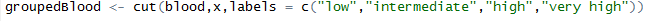
\includegraphics[width=0.8\textwidth]{RP2.png}
\end{center}
\caption{The use of the cut function in R for problem 2}
\end{figure}

\begin{figure}[h]
\begin{center}
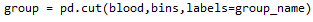
\includegraphics[width=0.6\textwidth]{PP2.png}
\end{center}
\caption{The use of the cut function in Python for problem 2}
\end{figure}

\newpage
\section*{References:}
\begin{enumerate}
\item{McKinney, Wes \emph{Python for Data Analysis}. O'Reilly Media Inc., 2013}
\item{(https://www.r-project.org/about.html).}
\item{(http://blog.datacamp.com/r-or-python-for-data-analysis/)}
\end{enumerate}

\end{document}